\RequirePackage{xcolor}
\documentclass[a4]{sciposter}
\usepackage{multicol,subfig,amsmath} % columnas, figuras, ecuaciones
\usepackage{graphicx,url,hyperref,doi}
\hypersetup{hidelinks} 
\usepackage[spanish]{babel}   
\usepackage[utf8]{inputenc}
\usepackage[sort&compress,numbers]{natbib}
\usepackage[font=small,labelfont=bf]{caption}
\usepackage[bottom]{footmisc}


\setlength{\parskip}{3pt} % espacio entre parrafos
\renewcommand{\arraystretch}{1.5} % altura de renglones de cuadros

\leftlogo[1.2]{img/UANL.png}
\rightlogo[1.2]{img/FIME.png} 

\title{Mejora de algoritmo de\\reconocimiento de emociones}
\author{Cecilia Jael Aguilar Aranda$^\dagger$,\\Alexander Espronceda Gómez$^\ddagger$\\Satu Elisa Schaeffer$^\ast$}
\institute {$^\dagger$Ingeniería en Administración de Sistemas,  $^\ddagger$Ingeniería en Tecnologías de Software, \\$^\ast$Posgrado en Ingeniería de Sistemas}
\email{$^\dagger$cecilia.aguilarand@uanl.edu.mx, $^\ddagger$alexander.esproncedago@uanl.edu.mx, $^\ast$elisa.schaeffer@uanl.edu.mx}


\begin{document}
\conference{\raisebox{0mm}[0cm]{
\includegraphics[width=80mm]{img/qr-code-Poster.png}}
  \raisebox{0mm}[0cm]{
\includegraphics[width=80mm]{img/qr-code-Project.png}}
  \hfill
  \raisebox{10mm}[0cm]{
\includegraphics[width=200mm]{img/Provericyt-2021.png}}
  \hfill
  \raisebox{10mm}[0cm]{
\includegraphics[width=200mm]{img/Verano-Logo.png}}
  }


\maketitle

\begin{abstract}
En este proyecto se busca incrementar el funcionamiento de un algoritmo de análisis de sentimiento en base a texto utilizando redes neuronales. Esto conlleva realizar modificaciones al código, así como el aumento del conjunto de datos con el que se trabaja. El objetivo es realizar un software conversacional capaz de reconocer patrones, determinar el sentimiento mostrado por el usuario y actuar acorde a ello.
\end{abstract}

\begin{multicols}{3} 

\section{Introducción}
El análisis de sentimiento se refiere a la aplicación de procesamiento de lenguaje natural, linguística computacional y análisis de texto para identificar la emoción del autor. \citep{definition}. En el presente documento se considera \textit{Análisis de sentimiento} y \textit{Reconocimiento de emociones} como un mismo concepto.

El objetivo principal de este proyecto es llevar a cabo diversos procesos que ayuden a que un algoritmo de análisis de sentimiento por medio de texto tenga un porcentaje de acierto más alto. Esto se logrará mediante búsqueda, análisis y filtrado de datos relevantes, así como también la actualización del algoritmo que está siendo utilizado actualmente.

\section{Antecedentes}
Este proyecto es parte del trabajo de tesis de \citet{chatbot}; se busca mejorar los resultados anteriormente obtenidos con la introducción de datos adicionales para el entrenamiento.

\begin{figure}
	\centering
	\captionsetup{type=figure}
	\setcounter{figure}{0}
	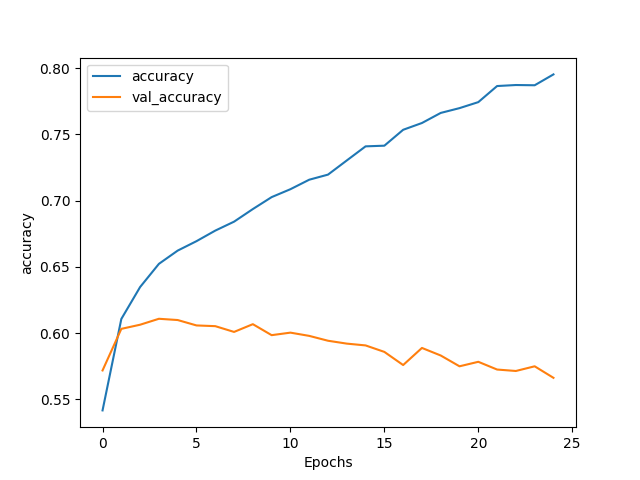
\includegraphics[scale=1.3]{img/Accuracy 2020-05_nofilter}
	\caption{Porcentaje de acierto del algoritmo, antes de aplicársele alguna mejora}
	
\end{figure}

\section{Estado de arte}

En la actualidad existen muchos algoritmos complejos de análisis de sentimiento que funcionan sin necesidad de introducir una cantidad excesiva de datos, tales como GPT-3 (Generative Pre-trained Transformer 3). En donde gracias a su uso eficiente de transformadores y también a que ha sido entrenado extensamente con conjuntos de datos enormes (por ejemplo: Wikipedia Corpus, Common Crawl, WebText2, entre otros), no hay necesidad de encontrar datos tan especificos para entrenarlos \citep{gpt3}.

La gran diferencia entre el algoritmo propuesto en este proyecto y algo más elaborado como lo es GPT-3, es el hecho de que este último no funciona localmente, sino que en realidad es una API por la cual se tiene que pagar para poder usar, además de que OpenAI posee completo control y regulación de los usos de su algoritmo \citep{openai}. 

Lo que se intenta hacer al momento de utilizar TensorFlow es darle el control completo al usuario en caso de que quiera darle sesgo a los datos o que lo adapte a las necesidades que tenga, sin necesidad de que pase a ser una caja negra. Este proceso es bastente complicado es posible que no se alcance el grado de porcentaje de acierto con el que cuenta GPT-3, pero se espera que sea lo suficiente como para poder ser una alternativa open-source viable.



\section{Solución propuesta}
La implementación se hizo en Python 3.7 \citep{python}, además de otras herramientas relacionadas con redes neuronales como Tensorflow 2.0.0 \citep{tensorflow} y procesamiento de lenguaje natural como NLTK \citep{nltk}


\paragraph{Metodología}
Se comienza por una búsqueda de conjuntos de datos para después filtrar las palabras que no aportan mucho significado al texto.

Se considera mejor un enfoque generalista debido a que las diferentes etiquetas de sentimiento a analizar no se encuentran distribuidas de manera uniforme; por lo que los datos se clasifican únicamente en \textit{"Bueno"},\textit{"Neutral"} y \textit{"Malo"}.

Se utiliza un algoritmo bidireccional STM con una activación de softmax de última capa. El léxico está limitado a 5000 elementos, y el largo máximo de cualquier frase después de ser filtrada es de 30 caracteres.

Ya después de ser actualizado, el conjunto de datos utilizado cuenta con alrededor de 60,000 tweets filtrados y clasificados.

Durante la fase de entrenamiento, se utilizaron 25 epochs con un 75\% del conjunto de datos en un orden arbitrario, usando el 25\% restante como validación.

\begin{figure}
	\centering
	\captionsetup{type=figure}
	\setcounter{figure}{1}
	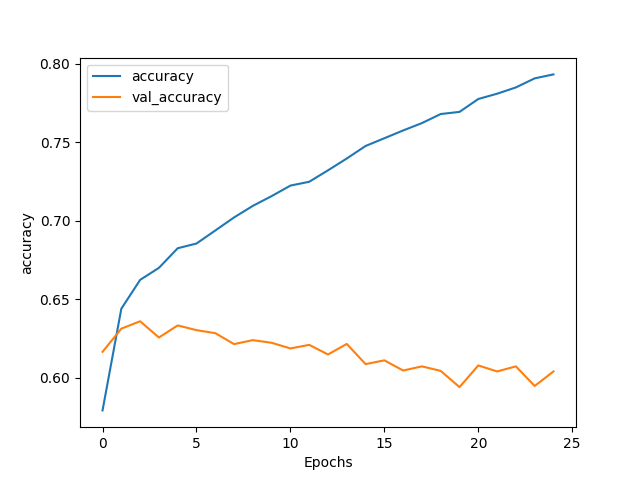
\includegraphics[scale=1.3]{img/Accuracy 2021-07.png}
	\caption{Porcentaje de acierto del algoritmo, después de aplicársele las mejoras propuestas}	
\end{figure}

\section{Experimentos}
Para examinar el impacto del enfoque propuesto, se realizaron múltiples ejecuciones del algoritmo con diferentes parámetros dentro de él, identificando áreas de oportunidad en donde se pueden hacer mejoras, para finalmente comparar resultados.



\begin{figure}[!tbp]
\captionsetup{type=figure}


  \centering
  \begin{minipage}[b]{0.45\textwidth}
    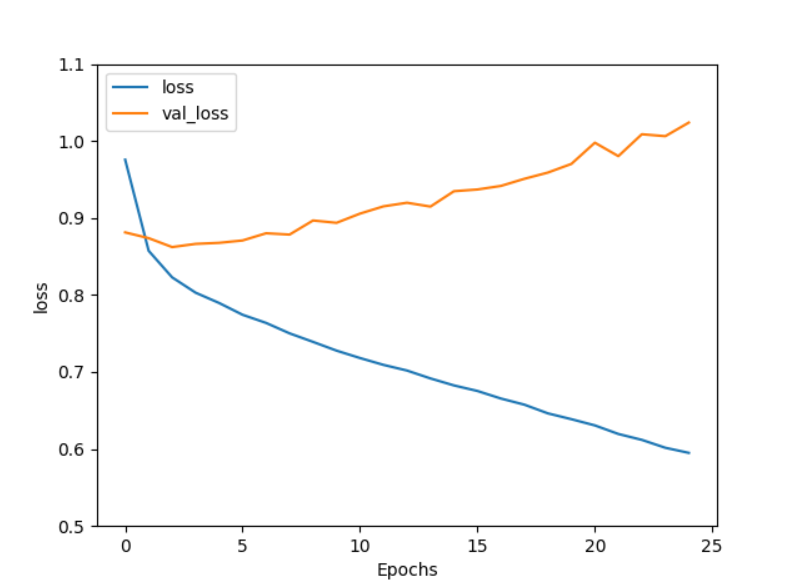
\includegraphics[width=1.1\textwidth]{img/Loss Before.png}
    \captionof*{figure}{a) Antes}
  \end{minipage}
  \begin{minipage}[b]{0.45\textwidth}
    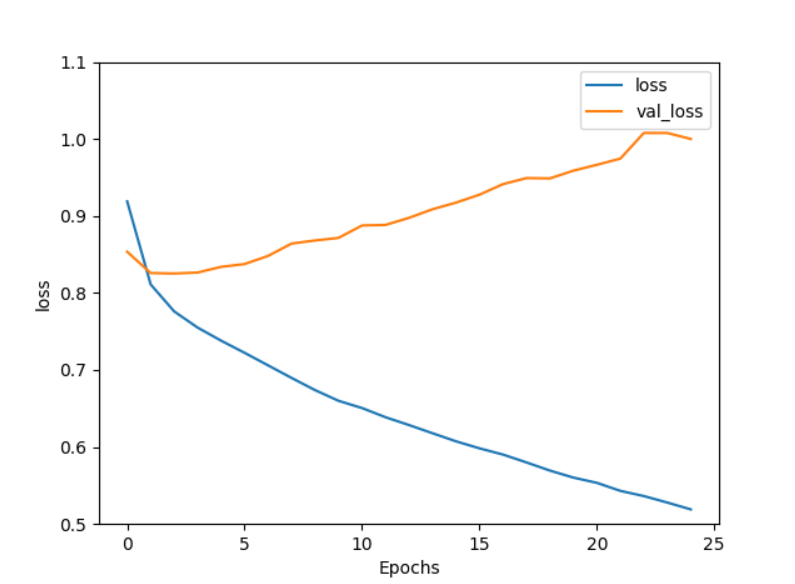
\includegraphics[width=1.1\textwidth]{img/Loss After.png}
    \captionof*{figure}{b) Después}
  \end{minipage}
  \caption{Pérdida antes y después de aplicarse la mejora}
\end{figure}



\begin{table}
\setcounter{table}{0} % por culpa de sciposter
\captionsetup{type=table} % por culpa de sciposter
\caption{Resultados de la precisión en los experimentos antes y después de aplicarse la mejora}
\label{data}
\begin{center}
\scalebox{0.9}{\begin{tabular}{|r|c|l|}
    \hline
         \multicolumn{1}{|c|}{}
         & \multicolumn{1}{|c|}{\rotatebox{90}{\bf Entrenamiento }}
         & \multicolumn{1}{|c|}{\rotatebox{90}{\bf Testeo\phantom{m}}} \\
         \hline
         \bf{Antes} & 80.64\% & 55.92\% \\
         \hline
         \bf{Después} & 81.75\% & 59.89\% \\
        \hline
    \end{tabular}}
\end{center}
\end{table}

\section{Conclusiones}

Se ha logrado un aumento en la precisión de reconocimiento de emociones, se espera realizar más modificaciones para mejorar el algoritmo y en un futuro implementarlo para su uso.

\paragraph{Agradecimientos}

{\small El primer autor agradece a PROVERICYT al dar la oportunidad de participar en el Verano de Investigación Científica y Tecnológica 2021 y proporcionar una beca.
El póster se preparó con \url{https://www.overleaf.com/}.}
\end{multicols}

\bibliography{poster}
\bibliographystyle{unsrtnat}



\end{document}
